\chapter{Introduction}

\section{Overview}

The Embedded Multicore Building Blocks (\embb) are an easy to use yet powerful and efficient C/C++ library for the development of parallel applications. \embb has been specifically designed for embedded systems and the typical requirements that accompany them, such as real-time capability and constraints on memory consumption. As a major advantage, low-level operations are hidden in the library which relieves software developers from the burden of thread management and synchronization. This not only improves productivity of parallel software development, but also results in increased reliability and performance of the applications.

\embb is independent of the hardware architecture (x86, ARM, ...) and runs on various platforms, from small devices to large systems containing numerous processor cores. It builds on MTAPI, a standardized programming interface for leveraging task parallelism in embedded systems containing symmetric or asymmetric multicore processors. A core feature of MTAPI is low-overhead scheduling of fine-grained tasks among the available cores during runtime. Unlike existing libraries, \embb supports task priorities, which allows the creation of soft real-time systems. Additionally, the scheduling strategy can be optimized for non-functional requirements such as minimal latency and fairness.

Besides the task scheduler, \embb provides basic parallel algorithms, concurrent data structures, and skeletons for implementing stream processing applications (see Figure~\ref{fig:introduction_embb_components}). These building blocks are largely implemented in a non-blocking fashion, thus preventing frequently encountered pitfalls like lock contention, deadlocks, and priority inversion. As another advantage in real-time systems, the algorithms and data structures give certain progress guarantees. For example, wait-free data structures guarantee system-wide progress which means that every operation completes within a finite number of steps independently of any other concurrent operations on the same data structure.

\begin{figure}[H]
  \centering
  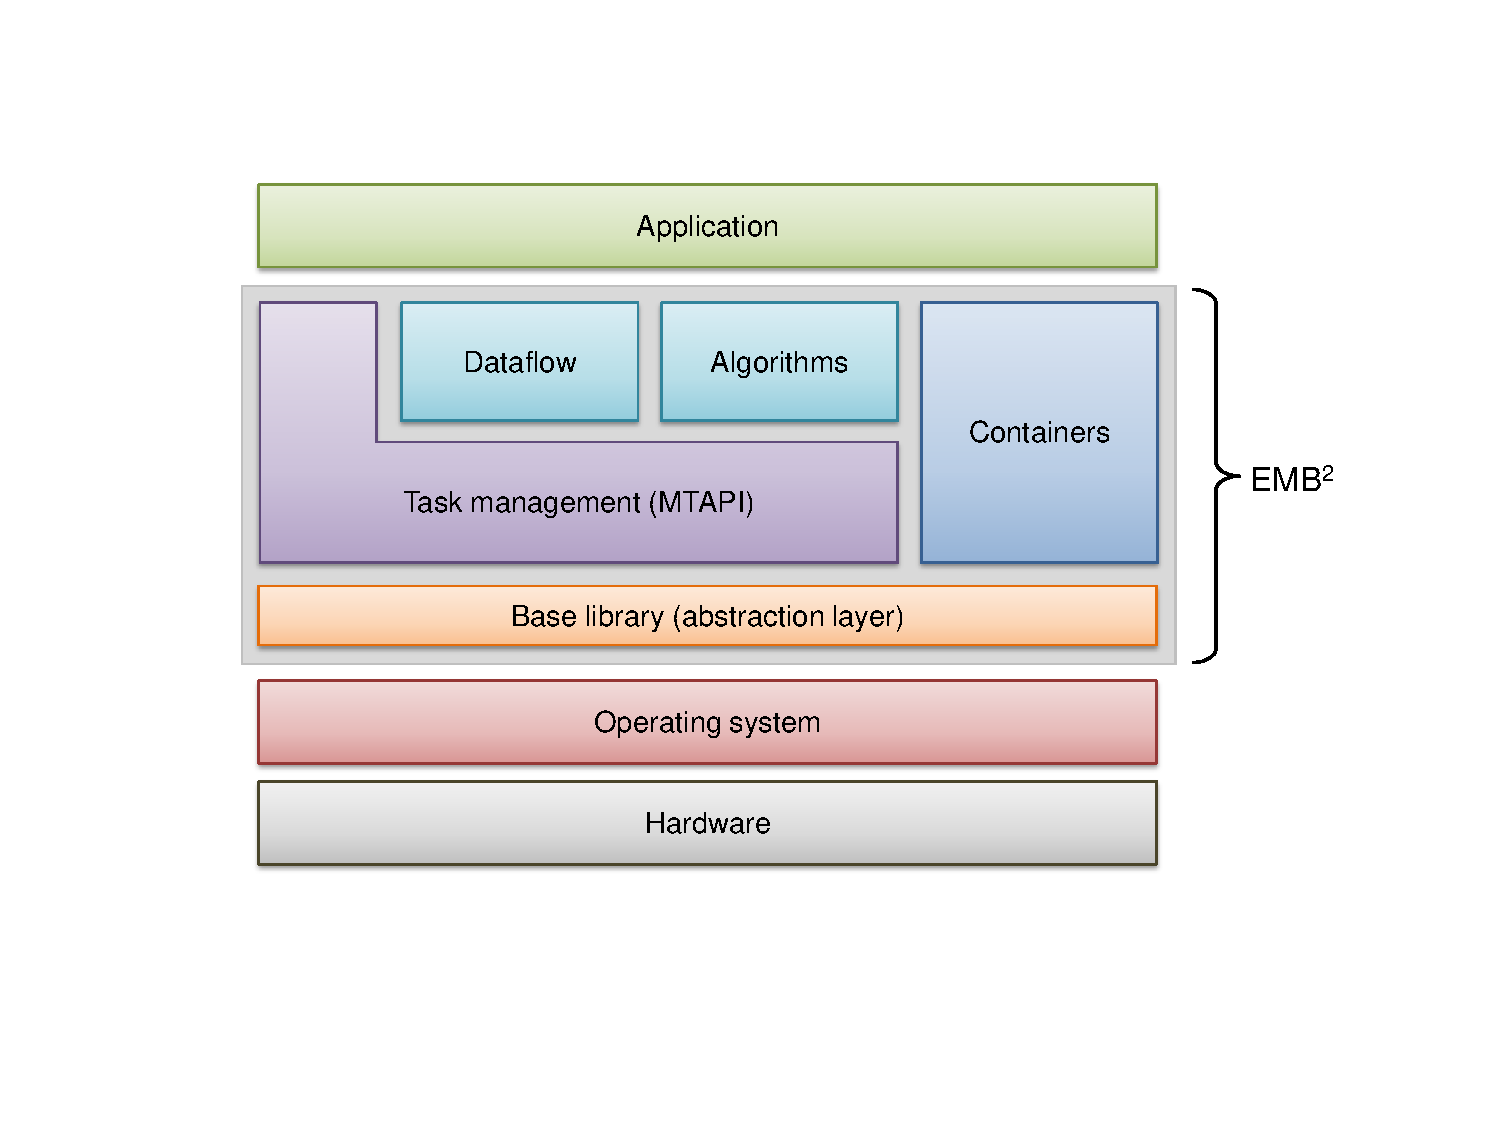
\includegraphics[width=0.75\columnwidth]{../images/embb.pdf}
  \label{fig:embb_components}
  \caption{Main building blocks of \embb}
  \label{fig:introduction_embb_components}
\end{figure}

% TODO
%\section{Key Features and Requirements}

\section{Outline}

The purpose of this tutorial is to introduce the basic concepts of \embb and to demonstrate typical application scenarios by means of simple examples. The tutorial is not intended to be complete in the sense that it describes every feature of \embb. For a detailed description of the API, please see the HTML documentation.

In the next subsection, we briefly describe the concept of function objects which is essential for using \embb. In Chapter~\ref{cha:mtapi}, we then present the task management features of MTAPI. These provide the basis for the algorithms outlined in Chapter~\ref{cha:algorithms} and the dataflow framework presented in Chapter~\ref{cha:dataflow}.

\section{Functions, Functors, and Lambdas}
\label{sec:introduction_function_objects}

Throughout this tutorial, we will encounter C++ types which model the C++ concept\footnote{In this context, the term \emph{concept} refers to a named set of requirements on a type.} \lstinline|FunctionObject|. The function object concept comprises function pointer, functor, and lambda types that are callable with suitable arguments by the function call syntax. Given a function object \lstinline|f| and arguments \lstinline|arg1|, \lstinline|arg2|, \lstinline|...|, the expression \lstinline|f(arg1, arg2, ...)| is a valid function invocation. If you are already familiar with function objects, you can safely skip the rest of this section. Otherwise, it might be worth reading it to get an idea of what is meant when talking about a function objects.

Consider, for example, the transformation of an iterable range of data values. Specifically, consider a vector of integers initialized as follows:
%
\\\inputlisting{../examples/stl_for_each/setup-snippet.h}
%
The range consists of the values (\lstinline|1, 2, 3, 4, 5|) and we now want to double each of them. We could simply get an iterator from the container holding the range, iterate over every element, and multiply it by two:
%
\\\inputlisting{../examples/stl_for_each/manual-snippet.h}
%
The range then contains the values (\lstinline|2, 4, 6, 8, 10|). In order to demonstrate the concept of function objects, we are now going to use the \lstinline|std::for_each| function defined in the \lstinline|algorithm| header of the C++ Standard Library. This function accepts as argument a \lstinline|UnaryFunction|, that is, a function object which takes only one argument. In case of \lstinline|std::for_each|, the argument has to have the same type as the elements in the range, as these are passed to the unary function. In our example, the unary function's task is to double the incoming value. We could define a function for that purpose:
%
\\\inputlisting{../examples/stl_for_each/function_define-snippet.h}
%
Since a function pointer models the concept of function objects, we can simply pass \lstinline|&DoubleFunction| to \lstinline|std::for_each|:
%
\\\inputlisting{../examples/stl_for_each/function-snippet.h}
%
Another possibility is to define a functor
%
\\\inputlisting{../examples/stl_for_each/functor_define-snippet.h}
%
and to pass an instance of this class to \lstinline|std::for_each|:
%
\\\inputlisting{../examples/stl_for_each/functor-snippet.h}
%
Functors as well as the function pointers separate the actual implementation from its place of usage which can be useful if the functionality is needed at different places. In many cases, however, it is advantageous to have the implementation of the function object at the same place as it is used. C++11 provides lambda expressions for that purpose which make our example more concise:
%
\\\inputlisting{../examples/stl_for_each/lambda-snippet.h}
%
Of course, this example is too simple to really benefit from function objects and the algorithms contained in the C++ Standard Library. However, in combination with the parallelization features provided by \embb, function objects are a helpful mechanism to boost productivity. Within this document, whenever a function object or one of its subtypes is required, one can use a function pointer, a functor, or a lambda. For simplicity, we will restrict ourselves to lambdas in subsequent examples, as they are most suitable for this kind of tutorial.
